\documentclass[Ingles]{assets/template/ic-tese-v3}
%\documentclass[Ingles,Final]{assets/template/ic-tese-v3}

\usepackage[latin1,utf8]{inputenc}

\usepackage[
    pdfauthor={Daniel De Lucca Fonseca},
    pdftitle={titulo},
    pdfkeywords={palavra-chave, palavra-chave},
    pdfproducer={Latex with hyperref},
    pdfcreator={pdflatex},
]{hyperref}

% Remover antes da versão final
\usepackage[
    draft,
%final,
]{changes}

\usepackage[printonlyused]{acronym}

\usepackage{amsmath}

\usetikzlibrary{shadows, arrows.meta, positioning}

\usepackage{listings}
\usepackage{xcolor}

\definecolor{codegray}{rgb}{0.5,0.5,0.5}
\definecolor{codeorange}{rgb}{0.8,0.3,0}
\definecolor{codeblue}{rgb}{0.2,0.2,0.6}

\lstdefinestyle{common}{
    basicstyle=\ttfamily\footnotesize,
    keywordstyle=\color{codeblue},
    commentstyle=\color{codegray}\itshape,
    stringstyle=\color{codeorange},
    showstringspaces=false,
    breaklines=true,
    frame=single,
    numbers=left,
    numberstyle=\tiny\color{codegray},
    captionpos=b,
    tabsize=2
}

\lstdefinestyle{pythonstyle}{
    style=common,
    language=Python
}

\lstdefinestyle{bashstyle}{
    style=common,
    language=bash,
    morekeywords={docker, echo, for, in, do, done, if, then, fi},
}

\usepackage{subcaption}
\usepackage{multirow}

\begin{document}
    \autor{Daniel De Lucca Fonseca}
    \titulo{Título da Dissertação ou Tese em Português}
    \title{The Dissertation or Thesis Title in English or Spanish}
    \orientador{Prof. Dr. Edson Borin}
    \mestrado
    \datadadefesa{22}{04}{2025}

% Para a versão final defina:
%\avaliadorA{Prof. Dr. Primeiro Avaliador}{Instituição do primeiro avaliador}
%\avaliadorB{Profa. Dra. Segunda Avaliadora}{Instituição da segunda avaliadora}
%\avaliadorC{Dr. Terceiro Avaliador}{Instituição do terceiro avaliador}
%\avaliadorD{Prof. Dr. Quarto Avaliador}{Instituição do quarto avaliador}
%\avaliadorE{Prof. Dr. Quinto Avaliador}{Instituição do quinto avaliador}
%\avaliadorF{Prof. Dr. Sexto Avaliador}{Instituição do sexto avaliador}
%\avaliadorG{Prof. Dr. Sétimo Avaliador}{Instituição do sétimo avaliador}
%\avaliadorH{Prof. Dr. Oitavo Avaliador}{Instituição do oitavo avaliador}

% Para incluir a ficha catalográfica em PDF na versão final, descomente e ajuste:
%\fichacatalografica{arquivo.pdf}

    \paginasiniciais

    % Definição dos autores
\definechangesauthor[name={Edson Borin}, color=purple]{EB}
\definechangesauthor[name={Daniel Fonseca}, color=red]{DF}

% Borin (EB)
\newcommand{\EB}[1]{\comment[id=EB]{#1}} % Adiciona como comentário feito por EB
\newcommand{\EBH}[1]{\highlight[id=EB]{#1}} % Destaca o texto
\newcommand{\EBC}[2]{\EBH{#1} \comment[id=EB]{#2}} % Destaca e adiciona comentário
\newcommand{\EBADD}[1]{\added[id=EB]{#1}} % Adiciona texto
\newcommand{\EBRM}[1]{\deleted[id=EB]{#1}} % Remove texto
\newcommand{\EBRP}[2]{\replaced[id=EB]{#2}{#1}} % Substitui um texto pelo outro


% Edson's notes
% Daniel, mudei as macros por que não consegui adicionar comentários no rótulo de uma das tabelas com o modo anterior.
\renewcommand{\EB}[1]{{\textcolor{blue}{(EB: #1)}}}
\renewcommand{\EBH}[1]{{\hl{#1}}}
\renewcommand{\EBC}[2]{\EBH{#1}{\color{blue}(EB: #2)}}
\renewcommand{\EBADD}[1]{{\textcolor{blue}{#1}}}
\renewcommand{\EBRM}[1]{{\textcolor{lightgray}{(#1)}}}
\renewcommand{\EBRP}[2]{\EBRM{#1}\EBADD{#2}}
\newcommand{\EBRPD}[2]{#1 \EB{#1 $\rightarrow$ #2?}}

% Daniel (DF)
\newcommand{\DF}[1]{\comment[id=DF]{#1}} % Adiciona como coomentário feito por DF
\newcommand{\DFH}[1]{\highlight[id=DF]{#1}} % Destaca o texto
\newcommand{\DFC}[2]{\DFH{#1} \comment[id=DF]{#2}} % Destaca e adiciona comentário
\newcommand{\DFADD}[1]{\added[id=DF]{#1}} % Adiciona texto
\newcommand{\DFRM}[1]{\deleted[id=DF]{#1}} % Remove texto
\newcommand{\DFRP}[2]{\replaced[id=DF]{#2}{#1}} % Substitui um texto pelo outro
\newcommand{\DFTODO}[1]{\DFADD{TODO: #1}} % Adiciona um TODO com comentário
    \prefacesection{Dedicatória}
As dedicatórias devem ter apenas uma página.
\DFTODO{Escrever a dedicatória}
    \begin{epigrafe}{
    \it
    Vita brevis,\\
    ars longa,\\
    occasio praeceps,\\
    experimentum periculosum,\\
    iudicium difficile.\\
    \DFADD{Preciso fazer a epígrafe}
}

\hfill (Hippocrates)
\end{epigrafe}
    \prefacesection{Agradecimentos}
Os agradecimentos devem ocupar uma única página.
\DFTODO{Escrever os agradecimentos}
    % Sempre deve haver um resumo em português:
\begin{resumo}
    O resumo deve ter no máximo 500 palavras e deve ocupar uma única página.
    \DFTODO{Escrever o resumo}
\end{resumo}

\begin{abstract}
    The abstract must have at most 500 words and must fit in a single page.
    \DFTODO{Escrever o abstract}
\end{abstract}
    \prefacesection{List of Acronyms}

\begin{acronym}
    \acro{HPC}{High Performance Computing}
    \acro{GC}{Garbage Collector}
    \acro{COW}{Copy-On-Write}
    \acro{RSS}{Resident Set Size}
    \acro{VMS}{Virtual Memory System}
    \acro{UNICAMP}{Universidade Estadual de Campinas}
    \acro{GST3D}{Generalized S-transform in 3D}
    \acro{RAM}{Random Access Memory}
    \acro{OS}{Operating System}
    \acro{I/O}{Input/Output}
    \acro{CPU}{Central Processing Unit}
    \acro{API}{Application Programming Interface}
    \acro{macOS}{Macintosh Operating System}
    \acro{DDR4}{Double Data Rate 4}
    \acro{GB}{Gigabyte}
    \acro{GPU}{Graphics Processing Unit}
    \acro{3D}{Three-Dimensional}
    \acro{OOM}{Out Of Memory}
    \acro{GST3D}{Gradient Structure Tensor 3D}
    \acro{RMSE}{Root Mean Square Error}
    \acro{MAE}{Mean Absolute Error}
    \acro{PBS}{Portable Batch System}
    \acro{SEG-Y}{Society of Exploration Geophysicists - Format Y}
    \acro{dind}{Docker-in-Docker}
    \acro{CSV}{Comma-Separated Values}
    \acro{XGBoost}{Extreme Gradient Boosting}
    \acro{MLP}{Multi-Layer Perceptron}
    \acro{GB}{Gigabyte}
    \acro{RTX}{Ray Tracing eXtreme}
    \acro{UNICAMP}{Universidade Estadual de Campinas}
    \acro{CV}{Coefficient of Variation}
    \acro{QQ}{Quantile-Quantile}
\end{acronym}
    \prefacesection{List of Symbols}

\newcommand{\T}{$T$}
\newcommand{\Mpeak}{$M_{\text{peak}}$}
\newcommand{\Mt}{$M(t)$}

\begin{table}[h]
    \centering
    \begin{tabular}{|l|c|p{5cm}|}
        \hline
        \textbf{Symbol} & \textbf{Description}   & \textbf{Description}                                                                                                \\ \hline
        \T              & Execution Time         & A metric which represents the total time, measured in seconds, taken for the execution of a task.                   \\ \hline
        \Mpeak          & Peak Memory Usage      & A metric which denotes the highest memory consumption observed during the execution of a task, measured in \ac{MB}. \\ \hline
        \Mt             & Memory Usage over Time & A metric which eflects the continuous tracking of memory consumption as a function of time throughout the task.     \\ \hline
    \end{tabular}
    \caption{Summary of all symbols used in this thesis}
    \label{tab:summary-of-symbols}
\end{table}

    \listoffigures
    \listoftables

    \tableofcontents

    \fimdaspaginasiniciais

    \chapter{Introduction}
\label{ch:introduction}


\section{Motivation}
\label{sec:intro-motivation}

\DFTODO{Desafios no processamento de dados em larga escala, focando em sísmica}
\DFTODO{Problemas com o gerenciamento de recursos em sistemas distribuídos como o Dask}
\DFTODO{A necessidade de prever o consumo de memória para definir o tamanho do chunk em algoritmos que são memory-intensive}


\section{Objectives}
\label{sec:intro-objectives}

\DFTODO{Desenvolver um método para estimar o consumo de memória com a menor quantidade de execuções possíveis}
\DFTODO{Tornar o auto-chunking do Dask memory-aware para reduzir a tentativa e erro na alocação de recursos}


\section{Contributions}
\label{sec:intro-contributions}

\DFTODO{Criação de um modelo preditivo para o consumo de memória}
\DFTODO{Desenvolvimento de um método para estimar o consumo de memória com poucas execuções}
    \chapter{Fundamental Concepts}
\label{ch:fundamental-concepts}

\DFTODO{Definir os conceitos fundamentais que serão explicados}
    \chapter{Related Work}
\label{ch:related-work}

\DFTODO{Definir os trabalhos relacionados que serão discutidos neste capítulo}
    \chapter{Measuring Memory Consumption of Python Programs}
\label{ch:measuring-memory-consumption}


\section{Introduction}
\label{sec:mmc-introduction}

Accurately measuring the memory consumption of Python programs is a fundamental aspect of performance analysis, especially in the context of scientific computing and data analysis workflows.
Scientific applications often involve large-scale computations, high-dimensional datasets, and complex algorithms that necessitate the use of \ac{HPC} environments such as supercomputers and distributed systems.
In these environments, resource allocation is a critical factor, directly impacting both computational efficiency and cost-effectiveness.
Understanding the memory usage patterns of applications enables researchers and engineers to allocate appropriate resources, optimize computational workflows, and prevent system-level bottlenecks.

In scientific workflows, the need for precise memory measurement extends beyond mere resource allocation.
Memory profiling is instrumental in identifying inefficiencies, diagnosing performance issues, and ensuring the scalability of algorithms across diverse computational environments.
Although this thesis primarily focuses on the execution of scientific workflows rather than their optimization, the accurate measurement of memory consumption remains pivotal.
Without precise memory metrics, the evaluation of algorithmic performance and the reproducibility of experimental results can be significantly compromised.

\subsection{Factors Affecting Memory Consumption Evaluation}
\label{subsec:mmc-factors-affecting-memory-consumption-evaluation}

The evaluation of memory consumption in Python applications is influenced by a multitude of factors spanning both the language's inherent characteristics and the underlying operating system's behavior.
Python, as a high-level language, abstracts many low-level memory management operations, introducing complexities that can obscure the true memory footprint of an application.

\begin{enumerate}
    \item \textbf{Dynamic Memory Allocation}:
    Python's memory model relies heavily on dynamic memory allocation, facilitated by its internal memory manager.
    The interpreter frequently allocates and deallocates memory for objects, leveraging techniques such as reference counting and cyclic garbage collection.
    These mechanisms introduce variability in memory usage, as memory may not be immediately released upon object deletion, leading to transient peaks in memory consumption.

    \item \textbf{Garbage Collection}:
    Python employs a \ac{GC} to manage memory, particularly for cyclic references that reference counting alone cannot handle.
    The \ac{GC} operates in generational cycles, triggering collections based on thresholds related to object allocations and deallocations.
    The timing of these collections can significantly affect memory profiling, as delayed garbage collection may artificially inflate memory usage metrics.

    \item \textbf{Memory Fragmentation}:
    Both Python's memory allocator (e.g., pymalloc~\cite{pymalloc}) and the underlying C libraries can cause memory fragmentation.
    Fragmentation leads to inefficient memory utilization, where the allocated memory space cannot be fully utilized due to non-contiguous free blocks.
    This phenomenon can result in higher apparent memory usage than the actual data footprint.

    \item \textbf{Operating System Optimizations}:
    Modern operating systems implement various memory management optimizations, such as virtual memory, \ac{COW}, and memory compression.
    The virtual memory system abstracts physical memory, allowing processes to perceive a contiguous memory space.
    \ac{COW} mechanisms, often triggered during process forking, can complicate memory measurements by deferring actual memory duplication until modification occurs.
    Additionally, features like Linux's zswap~\cite{zswap} and zram~\cite{zram} compress memory pages to optimize \ac{RAM} usage, further obscuring accurate memory accounting.

    \item \textbf{Caching Mechanisms}:
    Python and the operating system both employ caching strategies that can skew memory usage metrics.
    For instance, Python maintains internal caches for frequently used objects (e.g., small integers and strings), while the \ac{OS} uses disk and memory caches to optimize \ac{I/O} operations.
    These caches can persist across program executions, leading to inconsistent memory profiles unless explicitly cleared.

    \item \textbf{Third-Party Libraries}:
    Scientific applications often rely on third-party libraries (e.g., NumPy~\cite{numpy}, pandas~\cite{pandas}, TensorFlow~\cite{tensorflow}), which may implement their own memory management strategies.
    These libraries, typically written in C or C++, interact directly with system memory, bypassing Python's \ac{GC}.
    Consequently, memory usage attributed to Python may not fully represent the actual consumption, necessitating specialized profiling tools to capture native allocations.
\end{enumerate}

\subsection{The Criticality of Precise Memory Measurement in Experiments}
\label{subsec:mmc-criticality-of-precise-memory-measurement}

Achieving precise memory measurement is a delicate and challenging task, particularly in experimental setups where even minor inconsistencies can introduce significant biases.
Inaccurate memory profiling can lead to erroneous conclusions about an algorithm's efficiency, scalability, and resource requirements.

One of the primary challenges is the accumulation of residual memory from previous executions.
This issue is especially pronounced in interactive environments like Jupyter~\cite{jupyter} notebooks, where code cells can be executed multiple times without restarting the kernel.
Each execution may leave behind allocated memory that is not immediately reclaimed, either due to lingering references or delayed garbage collection.
This residual memory inflates subsequent memory usage measurements, creating misleading results.

For example, consider a scenario where a data-intensive operation is repeatedly executed within a Jupyter notebook.
Even if the data structures are explicitly deleted using \texttt{del}, Python's \ac{GC} might not immediately free the associated memory, particularly if a reference exist in the notebook's global namespace or within closures.
Over time, this leads to cumulative memory bloat, distorting the true memory footprint of the operation.

Beyond interactive environments, process-level memory accumulation can occur when running batch scripts or automated workflows.
If multiple experiments are executed sequentially within the same process without proper memory isolation, residual allocations from earlier runs can affect subsequent measurements.
Techniques such as spawning isolated subprocesses for each experiment can mitigate this issue, ensuring clean memory states between runs.

Another critical consideration is the impact of measurement tools themselves.
Profiling tools, whether external (e.g., psutil~\cite{psutil}, resource~\cite{importlib_resources}) or internal (e.g., tracemalloc~\cite{tracemalloc}), introduce overhead that can influence the very metrics they aim to capture.
High-frequency sampling, for instance, increases \ac{CPU} and memory load, potentially skewing performance characteristics.
Moreover, tools that rely on instrumentation may alter code execution paths, subtly affecting memory allocation patterns.

To address these challenges, rigorous experimental protocols are essential.
This includes:

\begin{itemize}
    \item Isolating experiments in separate processes or containers to prevent cross-contamination of memory states.
    \item Resetting the environment (e.g., restarting the Python interpreter or Jupyter kernel) before each measurement to ensure a clean slate.
    \item Controlling external factors, such as disabling \ac{OS}-level caches or running benchmarks on dedicated, idle systems to minimize background noise.
    \item Using hybrid measurement techniques, combining high-level process metrics with low-level memory tracing for comprehensive profiling.
\end{itemize}

In conclusion, precise memory measurement is not merely a technical detail but a cornerstone of robust experimental methodology.
It underpins the reliability and validity of performance evaluations, guiding both theoretical insights and practical optimizations in scientific computing.


\section{Approaches to Measure Memory Consumption}
\label{sec:mmc-approaches}

When measuring memory consumption in Python programs, it is essential to distinguish between two broad categories of approaches: external measurement techniques and internal measurement techniques.
This classification helps clarify the scope and effectiveness of different methods, as each group offers unique insights into memory usage from different perspectives.

\begin{itemize}
    \item \textbf{External Measurement Approaches} involve monitoring memory usage from outside the Python runtime environment.
    These techniques interact directly with the operating system to gather data about process memory consumption.
    They are particularly effective for capturing the overall memory footprint of a program, including memory allocated by external libraries, system-level resources, and native code executed alongside Python.
    Examples include tools like psutil, the resource module, and accessing memory metrics from the Linux /proc~\cite{procfs} filesystem.

    \item \textbf{Internal Measurement Approaches}, on the other hand, operate within the Python runtime itself.
    These methods provide fine-grained visibility into Python-specific memory allocations, allowing developers to trace memory usage down to individual objects, code lines, or function calls.
    They are invaluable for identifying memory leaks, inefficient data structures, and understanding memory behavior at a granular level.
    The tracemalloc module is a prime example of an internal measurement approach.
\end{itemize}

The separation into these two categories is not arbitrary; it reflects the complementary nature of the information provided.
External tools offer a high-level, system-wide view of memory consumption, which is crucial for understanding how a Python program interacts with the broader operating environment.
In contrast, internal tools delve deep into Python’s memory management, offering detailed diagnostics that external tools cannot capture.

Combining both external and internal measurement techniques often yields the most comprehensive understanding of a program’s memory behavior.
External tools can detect overall memory growth trends and system resource usage, while internal tools can pinpoint the specific code responsible for memory allocation.
This dual approach is especially useful in scientific computing workflows, where performance optimization requires both macro-level monitoring and micro-level diagnostics.

\subsection{External Measurement Approaches}
\label{subsec:mmc-external-measurement-approaches}

\subsubsection{psutil}

The psutil library is a cross-platform tool that allows Python programs to access system details and process information, including memory usage.
It interacts with the operating system to retrieve real-time data about process memory, \ac{CPU} usage, and other system metrics.

psutil works by interfacing with \ac{OS}-level \ac{API}, such as /proc on Linux, the Windows \ac{API} on Windows systems, and system calls on \ac{macOS}.
It can report key memory metrics like:

\begin{itemize}
    \item \textbf{\ac{RSS}}:
    The portion of memory occupied by a process that is held in \ac{RAM}.

    \item \textbf{\ac{VMS}}:
    The total amount of virtual memory used by the process.

    \item \textbf{Shared Memory}:
    Memory shared with other processes.
\end{itemize}

psutil provides a comprehensive overview of system-wide and process-specific resource usage, making it a versatile tool for performance monitoring.

\subsubsection{resource Module}

The resource module is part of Python's standard library and offers a lightweight method to track resource usage of the current process.
It provides metrics such as maximum \ac{RSS}, which reflects the peak physical memory usage during the execution of the program.

Unlike psutil which can monitor ongoing memory usage, resource is primarily used for capturing peak memory usage at specific checkpoints in the code.
This makes it ideal for benchmarking and performance evaluations.

\subsubsection{/proc Filesystem}

On Linux systems, the /proc virtual filesystem provides detailed information about processes, including memory usage.
Accessing \texttt{/proc/[pid]/smaps} allows for fine-grained analysis of memory allocation.

The smaps file breaks down memory usage into categories such as:

\begin{itemize}
    \item \textbf{Private and Shared Memory}:
    Differentiates between private memory and memory shared with other processes.

    \item \textbf{Anonymous Pages}:
    Memory not backed by any file.

    \item \textbf{Heap and Stack Segments}:
    Detailed insights into dynamic memory allocations.
\end{itemize}

While powerful, this approach requires root access for detailed process information and involves parsing raw text files, which can add complexity.

\subsection{Internal Measurement Approaches}
\label{subsec:mmc-internal-measurement-approaches}

\subsubsection{tracemalloc}

tracemalloc is a built-in Python module designed for tracing memory allocations.
It hooks into Python's memory allocator to record the size and source of each allocation, capturing stack traces for memory usage hotspots.

Key features of tracemalloc include:

\begin{itemize}
    \item \textbf{Memory Snapshots}:
    Capturing snapshots of memory usage at different points in the program's execution.

    \item \textbf{Snapshot Comparisons}:
    Analyzing changes in memory usage between snapshots.

    \item \textbf{Tracking Allocation Sources}:
    Identifying the specific lines of code responsible for memory usage.

    \item \textbf{Filtering and Grouping}:
    Aggregating memory statistics based on filenames, line numbers, or function calls.
\end{itemize}

While tracemalloc introduces some overhead, its granularity makes it invaluable for debugging memory-related issues within Python applications.


\section{Materials and Methods}
\label{sec:mmc-materials-methods}

\subsection{Experiment Setup}
\label{subsec:mmc-experiment-setup}

All experiments were conducted on Node 9 of the \ac{UNICAMP} Discovery Lab, a high-performance Linux machine configured with the following hardware specifications:

\begin{itemize}
    \item \textbf{\ac{CPU}}:
    AMD Ryzen 7--5700X, featuring 8 physical cores and 16 logical threads.

    \item \textbf{Memory}:
    32 GB \ac{DDR4} \ac{RAM}.

    \item \textbf{GPU}:
    NVIDIA RTX 4090 with 24 \ac{GB} of dedicated \ac{GPU} memory.

    \item \textbf{\ac{OS}}:
    Linux \DFTODO{Adicionar a versão e detalhes do Kernel}.
\end{itemize}

This configuration was chosen to ensure robust computational performance, providing both \ac{CPU} and \ac{GPU} resources capable of handling large-scale data processing and memory-intensive workloads.

The experimental environment was containerized using Docker~\cite{docker}, ensuring consistency and isolation across all test runs.
The specific software stack includes:

\begin{itemize}
    \item \textbf{Python}:
    Version 3.13, running inside Docker containers.

    \item \textbf{Docker Engine}:
    Version \DFTODO{(insert version here)} for container management.

    \item \textbf{Libraries}:
    psutil, resource, tracemalloc, \DFTODO{Adicionar todas as dependências}, and custom scripts for memory monitoring.
\end{itemize}

Containerization allowed for precise control over the execution environment, eliminating the influence of background processes and system-level resource contention.

\subsection{Experimental Isolation Techniques}
\label{subsec:mmc-experimental-isolation-techniques}

To ensure the precision and reliability of the collected metrics, each experiment was executed in an isolated environment within a separate Docker container.
This approach was critical for eliminating potential interference from other processes, thereby ensuring that the memory consumption metrics reflected only the behavior of the specific algorithm under investigation.
By encapsulating each experiment within its own container, we effectively prevented shared memory interference between concurrent experiments, as Docker provides robust namespace isolation that keeps processes and their memory allocations distinct from one another.

Furthermore, the use of Docker allowed for precise control over resource allocation, including dedicated \ac{CPU} and memory limits for each container.
This ensured consistent computational environments across all experimental runs, minimizing variability caused by fluctuating resource availability.
Each container was initialized from a clean state, meaning no residual data, cached processes, or memory leaks from prior executions could influence the results.
This `stateless` execution model was essential for maintaining experimental integrity and reproducibility.

In addition to the internal monitoring mechanisms within each container, an external monitoring system was implemented outside the Docker environment.
This system was responsible for tracking the total memory usage of each Docker container in real-time, providing an independent verification layer for the memory metrics collected inside the container.
This dual-layer monitoring strategy enhanced the robustness of our data, allowing for cross-validation of memory usage statistics and ensuring the highest level of measurement accuracy.

\subsection{Selected Algorithms for the Experiment}
\label{subsec:mmc-selected-algorithms-for-the-experiment}

In order to comprehensively evaluate and compare different memory measurement techniques, we selected a diverse set of algorithms that represent both seismic-specific and general-purpose computational workloads.
The chosen algorithms vary in terms of computational complexity and memory requirements, enabling us to analyze memory behavior under different conditions.
This selection allows for the assessment of memory consumption patterns across a spectrum of tasks, from lightweight operations to computationally intensive processes.

The selected algorithms include:

\subsubsection{Envelope}

The \textbf{Envelope}\DFTODO{Adicionar referência do Envelope} algorithm is widely used in seismic processing to extract the instantaneous amplitude of a seismic signal.
It operates by calculating the magnitude of the analytic signal derived from the original seismic trace.
This algorithm is computationally lightweight and does not require significant memory resources, making it an ideal candidate for testing memory measurement techniques under less memory-intensive conditions.
Its simplicity allows for precise tracking of memory usage without interference from complex computational overhead.
By including the envelope algorithm, we aim to understand how memory measurement tools perform in scenarios with minimal memory demands, providing a baseline for comparison with more resource-intensive algorithms.

\DF{Vale a pena adicionar uma descrição detalhada de como o Envelope funciona e como ele foi implementado nos apêndices?}

\subsubsection{\ac{GST3D}}

The \textbf{\ac{GST3D}}\DFTODO{Adicionar referência do GST3D} algorithm is a time-frequency analysis method applied to three-dimensional seismic data.
Unlike the envelope algorithm, \ac{GST3D} is computationally heavy and memory-intensive.
It involves multiple transformations and extensive matrix operations across the entire seismic cube, leading to rapid memory consumption as the dataset size increases.
The high computational and memory demands of \ac{GST3D} make it an excellent choice for stress-testing memory measurement techniques.
By evaluating how different tools handle the memory footprint of \ac{GST3D}, we can gain valuable insights into their accuracy and performance under memory-constrained conditions.
This algorithm helps us identify the strengths and limitations of each memory measurement approach when dealing with complex seismic computations.

\DF{Vale a pena adicionar uma descrição detalhada de como o GST3D funciona e como ele foi implementado nos apêndices?}

\subsubsection{3D Gaussian Filtering}

To incorporate a non-seismic algorithm that still processes three-dimensional data, we selected \textbf{\ac{3D} Gaussian Filtering}\DFTODO{Adicionar referência ao Gaussian Filtering}.
This algorithm is commonly used in image and signal processing for data smoothing and noise reduction.
It performs convolution over a \ac{3D} array, applying a Gaussian kernel to average the values of neighboring elements.
While \ac{3D} Gaussian filtering is not as memory-intensive as \ac{GST3D}, it requires substantial computational resources due to the convolution operations, especially for large datasets.
This makes it an excellent candidate for evaluating memory measurement techniques in general-purpose computational contexts.
By analyzing memory consumption during the execution of \ac{3D]} Gaussian filtering, we can assess how well the measurement tools capture memory usage patterns in non-seismic, yet computationally demanding, scenarios.

\DF{Vale a pena adicionar uma descrição detalhada de como o 3D Gaussian Filtering funciona e como ele foi implementado nos apêndices?}

\subsubsection{Rationale for Algorithm Selection}

The selection of these three algorithms — Envelope, \ac{GST3D}, and \ac{3D} Gaussian Filtering — provides a balanced framework for evaluating memory measurement techniques.
Each algorithm represents a distinct category:

\begin{itemize}
    \item \textbf{Envelope}: Lightweight, seismic-specific, low memory demand.
    \item \textbf{\ac{GST3D}}: Heavy, seismic-specific, high memory demand.
    \item \textbf{\ac{3D} Gaussian Filtering}: General-purpose, moderate to high computational demand.
\end{itemize}

By testing these algorithms, we can observe how different memory measurement techniques perform across a range of computational workloads.
This approach enables us to identify measurement accuracy, overhead, and potential biases introduced by each tool in both simple and complex computational environments.
The goal is to determine which memory measurement techniques provide the most reliable and consistent results across diverse algorithmic contexts.

\subsection{Memory Measurement Techniques}
\label{subsec:mmc-memory-measurement-techniques}

To achieve a comprehensive understanding of memory consumption patterns, a combination of internal and external memory measurement techniques was employed.
Each technique offers unique insights into memory behavior, targeting different layers of the software and hardware stack.
To ensure the accuracy and reliability of the collected data, separate experiments were conducted for each tool, allowing for a detailed comparison of their results.
Additionally, the external Docker monitoring script was used as a validation mechanism to cross-check the consistency and correctness of the measurements obtained from the internal tools.

Internally, psutil was used to monitor process-specific memory metrics within each Docker container.
This library provides real-time tracking of key metrics, including the \ac{RSS}, which represents the portion of memory held in physical \ac{RAM}, and the \ac{VMS}, which indicates the total virtual memory allocated to the process.
The experiments involving psutil focused on continuously capturing these metrics throughout the execution of each algorithm to analyze dynamic memory usage patterns over time.

In parallel, the resource module from Python’s standard library was employed to capture peak memory usage during execution.
This tool reports the maximum \ac{RSS}, reflecting the highest memory consumption point during the experiment.
Unlike psutil which provides continuous monitoring, resource is particularly suited for benchmarking scenarios where peak memory usage is the primary focus.
Experiments using resource were designed to capture these peaks at key execution checkpoints.

To gain deeper insights into memory allocations within the Python runtime, tracemalloc was utilized.
This module hooks into Python’s memory allocator to trace allocation events at a granular level.
It captures memory snapshots at different stages of the program, enabling the comparison of memory states over time and the identification of potential memory leaks.
Experiments with tracemalloc focused on analyzing allocation patterns, tracking memory usage growth, and pinpointing specific code segments responsible for significant allocations.

At the system level, memory allocation data was gathered directly from the Linux /proc filesystem, specifically by querying the \texttt{/proc/[pid]/smaps} file.
This approach provided detailed insights into private, shared, and anonymous memory segments for each process.
The /proc experiments were designed to extract fine-grained memory allocation information from the operating system, offering a complementary perspective to the process-centric view provided by psutil and resource.

To validate the results obtained from these internal tools, a custom monitoring script was developed to interact with the Docker \ac{API}.
This script continuously queried Docker’s resource metrics in real time, capturing the total memory usage of each Docker container.
By monitoring resource consumption externally, this approach provided an independent verification layer that was critical for detecting discrepancies between the internal measurements.

This experimental design enabled a thorough comparison of the tools in terms of:

\begin{itemize}
    \item \textbf{Accuracy}:
    How closely the measurements align with the external Docker-based validation.

    \item \textbf{Granularity}:
    The level of detail provided by each tool, ranging from high-level process metrics to fine-grained object-level allocations.

    \item \textbf{Overhead}:
    The computational cost introduced by the measurement process itself, particularly relevant for tools like tracemalloc that require additional memory for tracking allocations.
\end{itemize}

By comparing the results from each tool against the Docker-based validation, discrepancies were identified and analyzed to understand the strengths and limitations of each approach.

To summarize, table~\ref{tab:mmc-memory-measurement-tools} provides an overview of the memory measurement techniques used, along with their corresponding validation approaches.
This table serves as a concise reference to compare the strengths and limitations of each method, highlighting how the external Docker monitoring was leveraged to ensure the reliability of the collected data.

\begin{table}[h]
    \centering
    \begin{tabular}{|l|p{7cm}|}
        \hline
        \textbf{Tool}           & \textbf{Description}                                                                            \\ \hline
        psutil                  & Monitors process-specific memory metrics (\ac{RSS}, \ac{VMS}) within containers.                \\ \hline
        resource                & Captures peak memory usage at defined execution checkpoints.                                    \\ \hline
        tracemalloc             & Traces Python object allocations to identify memory usage patterns.                             \\ \hline
        /proc Filesystem        & Directly queries the Linux kernel for detailed memory allocation data.                          \\ \hline
        External Docker Monitor & Uses a custom script interfacing with the Docker \ac{API} to track container-wide memory usage. \\ \hline
    \end{tabular}
    \caption{Summary of memory measurement tools}
    \label{tab:mmc-memory-measurement-tools}
\end{table}

\subsection{Collected Metrics}
\label{subsec:mmc-collected-metrics}

The experiments were designed to capture essential metrics that reflect both the performance and memory consumption patterns of the selected algorithms.
These metrics were chosen to provide a holistic view of computational efficiency, memory utilization, and execution dynamics.
The collected data serves as the foundation for subsequent analysis, enabling the identification of performance bottlenecks, memory inefficiencies, and potential areas for optimization.

Table~\ref{tab:mmc-collected-metrics} summarizes the key metrics collected during each experimental run.
The table includes the symbol used to represent each metric, along with a detailed description of its significance.

\begin{table}[h]
    \centering
    \begin{tabular}{|l|c|p{5cm}|}
        \hline
        \textbf{Metric}        & \textbf{Symbol} & \textbf{Description}                                                                                                                                                                                                    \\ \hline
        Execution Time         & \T              & Represents the total time, measured in seconds, taken for the completion of each experimental run. It provides insights into the overall efficiency and performance of the algorithm under different memory conditions. \\ \hline
        Peak Memory Usage      & \Mpeak          & Denotes the highest memory consumption observed during the experiment, measured in MBs. This metric is critical for assessing memory efficiency and determining the maximum resource requirements.                      \\ \hline
        Memory Usage over Time & \Mt             & Reflects the continuous tracking of memory consumption as a function of time throughout the experiment. This temporal profile helps identify memory spikes, leaks, and overall consumption patterns.                    \\ \hline
    \end{tabular}
    \caption{Summary of collected metrics for the memory consumption experiments}
    \label{tab:mmc-collected-metrics}
\end{table}

\subsection{Experiment Execution Workflow}
\label{subsec:mmc-experiment-execution-workflow}

The experimental workflow was meticulously designed to systematically measure memory consumption under controlled conditions.
The process began with the generation of random \ac{3D} matrices, each having varying shapes to simulate different data scenarios.
For each unique shape, three distinct datasets were created to ensure variability and improve the robustness of the analysis.
This diversity in data shapes and instances helped to better understand how memory consumption fluctuates under different input conditions.

Once the datasets were generated, they were stored on disk to ensure consistency across all experimental runs.
This step eliminated any variability that could arise from generating data on-the-fly, thereby maintaining uniform conditions for all algorithms tested.

The algorithm execution phase involved launching dedicated Docker containers for each experiment.
This approach ensured complete isolation, preventing resource interference from other processes and maintaining a clean execution environment.
Each container was configured to mount the corresponding dataset from the disk, ensuring the data was readily accessible during runtime.
The algorithms were designed to load the dataset into memory, perform the necessary computations, and terminate upon completion.
This clear-cut process flow minimized background operations that could otherwise skew memory usage measurements.

Throughout the execution, memory consumption was rigorously monitored using various measurement tools integrated within the container environment.
This continuous monitoring allowed for real-time tracking of memory usage, capturing both peak usage and dynamic fluctuations over the course of the algorithm's execution.
The collected data provided comprehensive insights into memory behavior, which was critical for subsequent analysis and performance evaluation.

To clearly summarize the workflow, table~\ref{tab:mmc-experimental-workflow} outlines each step of the experimental process, while figure~\ref{fig:mmc-experiment-workflow} provides a flowchart that visually illustrates it.

\begin{table}[h]
    \centering
    \renewcommand{\arraystretch}{1.4}
    \setlength{\tabcolsep}{10pt}
    \begin{tabular}{|>{\raggedright\arraybackslash}p{3.5cm}|>{\raggedright\arraybackslash}p{7cm}|}
        \hline
        \textbf{Step}       & \textbf{Description}                                                                                                                       \\ \hline
        Data Generation     & Random \ac{3D} matrices with varying shapes were generated, creating multiple datasets for each shape to ensure variability.               \\ \hline
        Data Storage        & The generated datasets were stored on disk to be accessed during each experiment.                                                          \\ \hline
        Algorithm Execution & For each algorithm, a dedicated Docker container was launched.                                                                             \\ \hline
        Memory Monitoring   & During execution, memory usage was continuously monitored using the specified tools to capture both peak and real-time memory consumption. \\ \hline
    \end{tabular}
    \caption{Summary of the memory consumption experiment workflow}
    \label{tab:mmc-experimental-workflow}
\end{table}

\begin{figure}[h]
    \centering
    \includegraphics[width=0.8\textwidth]{./assets/images/04-experiment-flowchart}
    \caption{Flowchart illustrating the memory consumption experiment workflow.}
    \label{fig:mmc-experiment-workflow}
\end{figure}

\subsection{Evaluation Methodology}
\label{subsec:mmc-evaluation-methodology}

The evaluation of the experimental results was conducted using a multi-faceted approach that integrates statistical analysis and validation techniques.
This comprehensive methodology ensures that the analysis is both rigorous and reliable, providing meaningful insights into memory usage patterns, performance trends, and the computational efficiency of the algorithms.

The primary focus of the evaluation was to analyze three key aspects: memory efficiency, performance trends over time, and execution performance.
Each of these aspects offers a unique perspective on the algorithms’ behavior when analyzed with different profiling tools, enabling a comprehensive evaluation of the strengths and limitations of various memory measurement techniques.

In addition to the primary analysis, two validation techniques were employed to verify the accuracy and reliability of the collected data.
These validation methods ensure that the metrics accurately reflect the actual resource usage and performance characteristics of the experiments.

Table~\ref{tab:mmc-evaluation-criteria} summarizes the evaluation criteria and validation techniques used in this study.

\begin{table}[h]
    \centering
    \begin{tabular}{|l|p{6cm}|}
        \hline
        \textbf{Evaluation Criteria}     & \textbf{Description}                                                                                                                                                                                                                                 \\ \hline
        Memory Efficiency                & Evaluates \Mpeak across different algorithms, datasets, and profiling tools. By comparing these values, we can identify the differences between each memory measurement technique.                                                                   \\ \hline
        Performance Trends               & Analyzes \Mt to detect temporal consumption patterns, such as sudden spikes, gradual increases (indicative of memory leaks), and periods of stable usage.                                                                                            \\ \hline
        Execution Performance            & Correlates memory consumption metrics with \T to assess the trade-offs between memory usage and processing speed, providing insights into computational efficiency.                                                                                  \\ \hline
        Cross-Validation with Docker API & Verifies the internal memory usage data by comparing it with external monitoring results obtained through the Docker \ac{API}. This comparison helps ensure the consistency and reliability of the internal memory measurements.                     \\ \hline
        Memory Constraint Validation     & Re-executes experiments under constrained memory conditions, with limits set slightly below the previously recorded \Mpeak. This validation confirms whether the measured \Mpeak represents the minimum memory requirement for successful execution. \\ \hline
    \end{tabular}
    \caption{Evaluation criteria and validation techniques for the memory consumption experiments}
    \label{tab:mmc-evaluation-criteria}
\end{table}

The cross-validation with Docker \ac{API} data provided an external benchmark to verify the accuracy of the internal memory measurements.
By comparing the internal data with Docker's resource metrics, we ensured that the recorded memory usage reflected the actual resource consumption of the containerized environments.

Furthermore, the memory constraint validation served as a practical test to confirm the robustness of the peak memory usage measurements.
By limiting the available memory to slightly below the recorded \Mpeak, we observed whether the algorithm could still execute successfully.
Failure to complete the execution under these constrained conditions validated that the original \Mpeak measurement accurately represented the minimum memory required for the algorithm to run without errors.

This comprehensive evaluation framework ensures that the analysis of memory consumption and performance is both thorough and reliable, providing meaningful insights into the behavior of the algorithms under various resource constraints.

\subsection{Experiment Repository}
\label{subsec:mmc-experiment-repository}

You can find all the code, results, and experimental data used in the following repository: \DFTODO{Adicionar o link pro repositório}.


\section{Experimental Results}
\label{sec:mmc-results}

\DFTODO{Demonstrar resultados dos experimentos com viés (sem controlar o ambiente). Mostrando o impacto de execuções anteriores}
\DFTODO{Apresentar os resultados dos experimentos, mostrando o consumo de memória e o tempo de execução para cada algoritmo.}
\DFTODO{Destacar a validação feita para garantir a precisão das medições. Encontrando a questão da pressão de memória}
\DFTODO{Demonstrar o impacto ao aplicar pressão de memória}


\section{Conclusion}
\label{sec:mmc-conclusion}

\DFTODO{Concluir a respeito da necessidade de ambientes controlados para medir a memória}
\DFTODO{Concluir sobre as diferentes formas de medir a memória}
\DFTODO{Concluir sobre o garbage collector e a possibilidade de executar com pressão de memória}
    \chapter{Predicting Memory Consumption from Input Shapes}
\label{ch:predicting-memory-consumption-from-input-shapes}

\section{Introduction}
\label{sec:pmc-introduction}

\ac{HPC} environments require users to specify computing resources, especially memory, before a job begins execution.
Common \ac{HPC} job schedulers, such as Slurm~\cite{yoo2003slurm} or \ac{PBS}~\cite{henderson1995pbs}, enforce fixed memory reservations at submission time.
This enforcement compels users to estimate a job's memory footprint in advance.
That requirement creates a fundamental challenge: users must predict memory needs \emph{a priori}, often without the benefit of trial runs.
Setting the memory request too low causes out-of-memory errors~\cite{bailey2005,hovestadt2003}, leading to lost computing time and queued tasks.
Setting it too high wastes memory and reduces overall system utilization because nodes retain unused allocations.
Accurate memory estimation therefore remains crucial for reliability and efficiency in \ac{HPC} resource management.

Most users rely on guesswork to determine memory reservations.
Many \ac{HPC} users adopt trial-and-error methods~~\cite{rodrigues2016,li2019,newaz2023,tanash2021ampro}, iteratively adjusting memory limits across repeated job submissions until one run completes without errors.
This approach leads to inefficiency and significant risk.
Each failed attempt wastes wall-clock time and computational cycles, while each successful run with excessive memory allocations deprives other jobs of available resources.
Over-provisioning represents a common workaround but leaves systems underutilized.
That trial-and-error paradigm reduces overall throughput and burdens users with resource-tuning responsibilities instead of scientific exploration.

Predictive modeling for memory allocation offers a clear path to improvement.
Models can forecast a job's memory demand using readily available workload features such as input data size, dimensionality, algorithmic parameters, or usage patterns from similar jobs.
These forecasts reduce guesswork and limit the need for iterative resubmissions.
More accurate pre-runtime memory predictions enable users to request memory more precisely, mitigating failure risks and alleviating resource waste~\cite{tanash2021ampro}.

The content in this chapter prioritizes tensor-based workloads, which revolve around large multidimensional arrays often referred to as \textit{tensors}.
For clarity, the term “tensor-based” (or equivalently, “tensor-centric”) describes computations centered on these large data structures, sometimes also called “array-based” workloads.
which exhibit strong correlations between memory usage and input shape.
Numerous scientific and data-centric applications center on these large multidimensional arrays.
Examples include seismic wave simulations on \ac{3D} grids, high-resolution image analysis in computer vision, and large-scale numerical linear algebra routines in scientific computing.
Memory consumption in these scenarios often scales according to array dimensions, because storage for input data structures and intermediate results typically dominates memory usage.
For example, doubling the resolution of an input image in each dimension roughly quadruples its memory footprint~\cite{stackoverflow_memory_inv}, while in deep neural networks increasing either input size or batch size similarly amplifies memory usage due to larger activation maps and additional computation~\cite{dell_3dunet_memory}.
These relationships underscore the crucial role of input shape in determining memory demands for tensor-centric workloads.
A predictive model that captures how memory scales with shape parameters can then offer robust estimates for new input configurations.

Several research directions have explored memory usage estimation and prediction in related fields.
In the \ac{HPC} domain, historical job data from systems like Slurm often enable machine learning models to predict resource consumption.
These models exploit features such as job metadata and input sizes to forecast memory requirements~\cite{yoo2003slurm}.
That approach demonstrates that ample historical data can support reliable predictions for recurring workloads.
In high-level numerical computing, analytical modeling of memory for array operations provides another possibility~\cite{cornell_memory_workshop}.
Matrix multiplications, convolutions, and other tensor-based methods can be studied to deduce peak memory usage without full execution.
Deep learning frameworks take a similar route to anticipate a network's memory footprint.
Layer-by-layer analysis of network architectures and input tensor dimensions reveals how memory usage accumulates~\cite{gao2020, dell_3dunet_memory}.
Profiling and simulation tools further assist deployment decisions by projecting memory usage before runtime~\cite{tanash2019}.

The primary objective of the present chapter is to estimate memory usage for new jobs given their input shapes, rather than to yield an exact byte-level measurement.
This emphasis on practical accuracy aims to provide a sufficiently precise estimate of peak memory demand to guide resource allocation.
Slight discrepancies arise due to overheads and system factors, but a well-calibrated predictor avoids severe underestimates that result in \ac{OOM} failures.
Focusing on a reliable upper-bound estimate allows users to reserve memory with greater confidence.
Narrowing the gap between requested and consumed memory improves performance over purely heuristic-based approaches and alleviates the risks and inefficiencies commonly associated with guesswork.
\section{Materials and Methods}
\label{sec:pmc-materials-and-methods}

This section explains the complete methodology for gathering memory-consumption data, generating shape-based features, and training predictive models.
The overall pipeline includes four core phases.
(i) Data Generation,
(ii) Memory Profiling,
(iii) Result Collection,
and (iv) Analysis.
These phases ensure consistent, reproducible, and high-quality measurements, which support machine learning models that learn memory usage from shape attributes.

\vspace{1em}
\noindent
\textbf{Phase 1: Data Generation.}
The experiment begins with synthetic seismic datasets.
In a typical seismic application, three dimensions describe the data: inlines, xlines, and samples.
The script systematically enumerates shape configurations by varying these dimensions from an \texttt{INITIAL\_SIZE} to a \texttt{FINAL\_SIZE} with increments of \texttt{STEP\_SIZE}.
For example, when the initial size equals 100, the final size equals 600, and the step size equals 100, the script generates volumes of sizes
\(\{\,(100,100,100),\,(100,100,200),\dots,(600,600,600)\}\)
and writes them to \ac{SEG-Y}~\cite{barry1975segy} files.
These synthetic datasets mimic actual seismic data and span diverse volumes to reveal how memory grows with increasing dimension sizes.

\vspace{1em}
\noindent
\textbf{Phase 2: Memory Profiling.}
A shell script schedules container-based jobs to run seismic operators on each generated dataset.
Chapter~\ref{ch:measuring-memory-consumption} describes the \ac{HPC}-like constraints and the rationale for isolating each job to reduce interference.
Accordingly, the script starts \ac{dind} containers pinned to specific \ac{CPU} cores through \texttt{--cpuset-cpus}.
This binding ensures comparable runs.
The script then processes three main operators:

\begin{itemize}
    \item \emph{Envelope}~\cite{taner1979complex}: A classic seismic attribute that computes instantaneous amplitude for each trace.
    \item \emph{\ac{GST3D}}~\cite{bigun2004recognition}: A structural attribute designed to highlight seismic faults or discontinuities.
    \item \emph{3D Gaussian Filter}~\cite{gonzalez2002digital}: A spatial smoothing operator for seismic volumes.
\end{itemize}

Each operator appears as a Docker image defined in the \texttt{Dockerfile}.
Each container execution uses a Python script to load and process input data.
The \texttt{traceq} library records \ac{RSS} over time, as discussed in Chapter~\ref{ch:measuring-memory-consumption}.
On completion, a \texttt{.prof} file stores the memory timeline and associated metadata, including timestamps and shape parameters.
This procedure captures peak memory usage accurately.

\vspace{1em}
\noindent
\textbf{Executing Operators and Gathering Profiles.}
Listing~\ref{lst:exp_sh} shows portions of the shell script.
The script orchestrates the sequence.
(i) create Docker volumes,
(ii) run a Python script to generate the synthetic datasets,
(iii) for every generated \ac{SEG-Y} file, execute Envelope, \ac{GST3D}, or Gaussian Filter,
(iv) run a Python script to parse and consolidate measurements,
and (v) finalize executing another Python script for exploratory data analysis.
Each run deposits output \ac{CSV} files and profiles in designated \texttt{OUTPUT\_DIR} subdirectories.

\vspace{1em}
\begin{lstlisting}[style=bashstyle,caption={Excerpts from \texttt{experiment.sh}~\cite{delucca2025experiment2script} that orchestrate Docker-based runs. Variables like \texttt{DATASET\_FINAL\_SIZE} and \texttt{DATASET\_STEP\_SIZE} define shape ranges for dataset generation.}, label={lst:exp_sh}]
#!/usr/bin/env sh
TIMESTAMP="$(date +%Y%m%d%H%M%S)"
CPUSET_CPUS="0"
DATASET_FINAL_SIZE="800"
DATASET_STEP_SIZE="50"

echo "Generating input data..."
docker run \
  --cpuset-cpus=0 \
  -v "${DIND_VOLUME_NAME}:/var/lib/docker:rw" \
  ...
  --env EXPERIMENT_COMMAND="generate_data.py" \
  --env EXPERIMENT_ENV="\
    -e OUTPUT_DIR=/experiment/out \
    -e FINAL_SIZE=${DATASET_FINAL_SIZE} \
    -e STEP_SIZE=${DATASET_STEP_SIZE} \
  " \
  docker:28.0.1-dind \
  "/workspace/experiment.sh"

echo "Collecting memory profile for Envelope..."
for file in "${OUTPUT_DIR}/inputs"/*.segy; do
  filename=$(basename "$file" .segy)
  docker run \
    --cpuset-cpus=0 \
    ...
    --env EXPERIMENT_COMMAND="collect_memory_profile.py" \
    --env EXPERIMENT_ENV="\
      -e ALGORITHM=envelope \
      -e INPUT_PATH=/experiment/out/inputs/${filename}.segy \
    " \
    docker:28.0.1-dind \
    "/workspace/experiment.sh"
done
...
\end{lstlisting}

\noindent
Table~\ref{tab:env_vars} summarizes relevant environment variables used by these scripts.
They control dataset sizes, repetition counts, and output paths.

\begin{table}[htbp]
    \centering
    \caption{Key environment variables for the experimental scripts.
    Defaults appear in parentheses.
    \vspace{1em}}
    \label{tab:env_vars}
    \begin{tabular}{ll}
        \hline
        \textbf{Variable}             & \textbf{Description}                                                                        \\
        \hline
        \texttt{DATASET\_FINAL\_SIZE} & Final dimension size (e.g., 800)                                                            \\
        \texttt{DATASET\_STEP\_SIZE}  & Step size between dimension increments (e.g., 50)                                           \\
        \texttt{EXPERIMENT\_N\_RUNS}  & Number of repeated runs per shape (e.g., 30)                                                \\
        \texttt{CPUSET\_CPUS}         & \ac{CPU} core pinning for Docker containers (e.g., 0)                                       \\
        \texttt{OUTPUT\_DIR}          & Directory for output profiles, logs, and \texttt{\ac{CSV}} files                            \\
        \texttt{ALGORITHM}            & Selected operator (e.g., \texttt{envelope}, \texttt{\ac{GST3D}}, \texttt{gaussian\_filter}) \\
        \hline
    \end{tabular}
\end{table}

\vspace{1em}
\noindent
\textbf{Phase 3: Results Collection and Feature Construction.}
This phase consists in evaluating the \texttt{.prof} files output by \texttt{traceq}, extracting peak memory usage, and associating it with the input shape.
The script identifies inlines, xlines, and samples from filenames, notes the operator, retains the maximum time-series \ac{RSS} value, and compiles a consolidated dataframe.
It also derives extended features such as total volume
(\(\text{inlines} \times \text{xlines} \times \text{samples}\)),
logarithmic transforms
(e.g., \(\log_2(\text{volume})\)),
surface area,
dimension ratios,
and polynomial expansions.
These features capture various ways shape correlates with peak memory usage.
Listing~\ref{lst:results_py} shows how this phase generates and transforms these features.

\begin{lstlisting}[style=pythonstyle,
    caption={Feature extraction excerpt from \texttt{collect\_results.py}~\cite{delucca2025experiment2resultscollection}. Additional derived metrics capture polynomial or ratio-based growth.},
    label={lst:results_py}]
df_features["volume"] = (
    df_features["inlines"]
    * df_features["xlines"]
    * df_features["samples"]
)

df_features["diagonal_length"] = np.sqrt(
    df_features["inlines"]**2
    + df_features["xlines"]**2
    + df_features["samples"]**2
)

df_features["surface_area"] = 2 * (
    df_features["inlines"] * df_features["xlines"]
    + df_features["inlines"] * df_features["samples"]
    + df_features["xlines"] * df_features["samples"]
)

df_features["log_inlines"] = np.log2(df_features["inlines"])
df_features["log_volume"] = np.log2(df_features["volume"])
...
\end{lstlisting}

\vspace{1em}
\noindent
\textbf{Phase 4: Model Training and Analysis.}
Phase 4 trains multiple regression models using inlines, xlines, samples, and derived features as predictors.
Peak memory usage serves as the target variable.
An 80/20 training/test split ensures fair comparisons across Envelope, \ac{GST3D}, and Gaussian Filter runs.

Four standard regression metrics evaluate model performance:
\ac{RMSE}~\cite{hyndman2006},
\ac{MAE}~\cite{willmott2005mae},
\(R^2\)~\cite{draper1998applied},
and a custom “accuracy” measure \(\mathrm{acc}\).
These metrics form a single optimization target:
\[
    \texttt{score} \;=\;
    w_\mathrm{acc}\,\cdot\,\mathrm{acc}
    \;-\;
    w_\mathrm{RMSE}\,\cdot\,\mathrm{RMSE}
    \;-\;
    w_\mathrm{MAE}\,\cdot\,\mathrm{MAE}
    \;+\;
    w_{R^2}\,\cdot\,R^2,
\]
where \(w_\mathrm{acc}, w_\mathrm{RMSE}, w_\mathrm{MAE},\) and \(w_{R^2}\) indicate how strongly the pipeline rewards or penalizes each metric.
Maximizing \(\texttt{score}\) balances the risk of underestimating memory (which can trigger job failures) against the cost of over-provisioning (which wastes resources).

The \texttt{Optuna} framework~\cite{akiba2019optuna} guides hyperparameter tuning for each model and determines suitable weights for \(\mathrm{acc}\), \(\mathrm{RMSE}\), \(\mathrm{MAE}\), and \(R^2\).
A study is created with \(\texttt{direction}=\text{"maximize"}\); at every trial, the study trains the model, evaluates the composite score, and updates search parameters accordingly.
The best trial parameters yield an optimal combination of hyperparameters and multi-metric weights.

Regarding models, the analysis includes several families of regressors:

\begin{itemize}
    \item \textbf{Linear Regression, Polynomial Regression}~\cite{hastie2009elements}\\
    These models create foundational baselines to capture the relationship between features and memory usage.
    Linear regression indicates whether memory usage scales directly with any of the features.
    Polynomial regression extends linear models with higher-order terms to account for mild nonlinearities.
    Caution is required since purely linear fits underfit complex relationships, and high-degree polynomials risk overfitting.

    \item \textbf{Decision Trees}~\cite{breiman1984classification}, \textbf{Random Forest}~\cite{breiman2001random}, \textbf{\ac{XGBoost}}~\cite{chen2016xgboost}\\
    \EB{Lembre-se de revisar a versão final para identificar e corrigir eventuais invasões de margem, como acima.}
    These tree-based methods automatically model complex feature interactions and nonlinearities.
    Decision Trees provide easy interpretability and can indicate shape thresholds that strongly affect memory.
    Random Forest aggregates multiple trees to reduce variance and enhance generalization.
    \ac{XGBoost} incrementally refines an ensemble of weak learners, which often results in higher accuracy on structured data.
    Hyperparameter tuning (e.g., tree depth or learning rate) is essential to avoid overfitting. \EB{Seria bom adicionar uma referência para dar suporte a este comentário.}

    \item \textbf{Neural Networks (\ac{MLP})}~\cite{rumelhart1986learning}\\
    \ac{MLP} architectures can approximate intricate functions when provided sufficient capacity.
    This property can reveal subtle relationships between shape parameters and memory requirements.
    These models often demand larger datasets, rigorous hyperparameter optimization, and careful overfitting control. \EB{Seria bom adicionar uma referência para dar suporte a este comentário.}

    \item \textbf{Gaussian Processes}~\cite{rasmussen2006gaussian}\\
    This approach offers both mean predictions and uncertainty estimates.
    Uncertainty bounds are especially valuable in \ac{HPC} scenarios where underestimating memory can cause abrupt job failures.
    Large datasets pose computational challenges because of the \(O(n^3)\) scaling, and kernels must be selected carefully. \EB{Seria bom adicionar uma referência para dar suporte a este comentário.}

    \item \textbf{Bayesian Ridge Regression}~\cite{bishop2006pattern}\\
    This extension of linear models applies Bayesian inference to estimate coefficients and yields robust predictions with uncertainty quantification.
    HPC workloads benefit from these uncertainty estimates when resource over-provisioning is less harmful than running out of memory.
    Polynomial or interaction terms might still be necessary to represent nonlinear growth patterns.
\end{itemize}

The script final Python script then visualizes memory distributions, residual plots, feature evaluations, and data-reduction experiments.
This exploration reveals each model’s generalization capacity, indicates which features add minimal value, and evaluates the number of training examples that the predictive framework requires.
Partial dependence plots and tree-based model interpretations expose how inlines, xlines, and samples exert the highest influence on memory usage.

\vspace{1em}
\noindent
\textbf{Technical Considerations.}
\begin{itemize}
    \item \emph{Containerization and Reproducibility:}
    Each stage runs in a Docker container with pinned versions of Python packages.
    This standardized environment preserves consistent results by preventing version drift.
    \item \emph{\ac{CPU} Affinity:}
    The \texttt{--cpuset-cpus=0} parameter restricts execution to a single core and reduces background noise.
    Multiple runs per dataset shape (\texttt{EXPERIMENT\_N\_RUNS}) further stabilizes performance measurements by smoothing out random fluctuations, often described as stochastic variance.
    \item \emph{Parallelization:}
    The Docker orchestration scales to multiple \ac{CPU} cores, but the design imposes single-core experiments for repeatability.
    Actual \ac{HPC} clusters manage concurrency at the scheduler level, but the core principle of shape-driven memory profiling remains applicable.
    \item \emph{Cache Handling:}
    Chapter~\ref{ch:measuring-memory-consumption} recommends dropping Linux memory caches to eliminate carry-over effects.
    This option appears in the scripts to ensure a clean environment for memory measurements.
\end{itemize}

\vspace{1em}
\noindent
Figure~\ref{fig:pmc_datapipeline} illustrates the entire workflow.
The process generates synthetic \ac{SEG-Y} volumes, runs containerized operators for memory profiling, and consolidates results into a final dataset that links shape features to peak memory usage.
Regression models then learn to map input dimensions to memory demand.
Section~\ref{sec:pmc-results} elaborates on these experimental outcomes and compares the predictive accuracy of the considered models.

\begin{figure}[htbp]
    \centering
    \resizebox{\textwidth}{!}{
        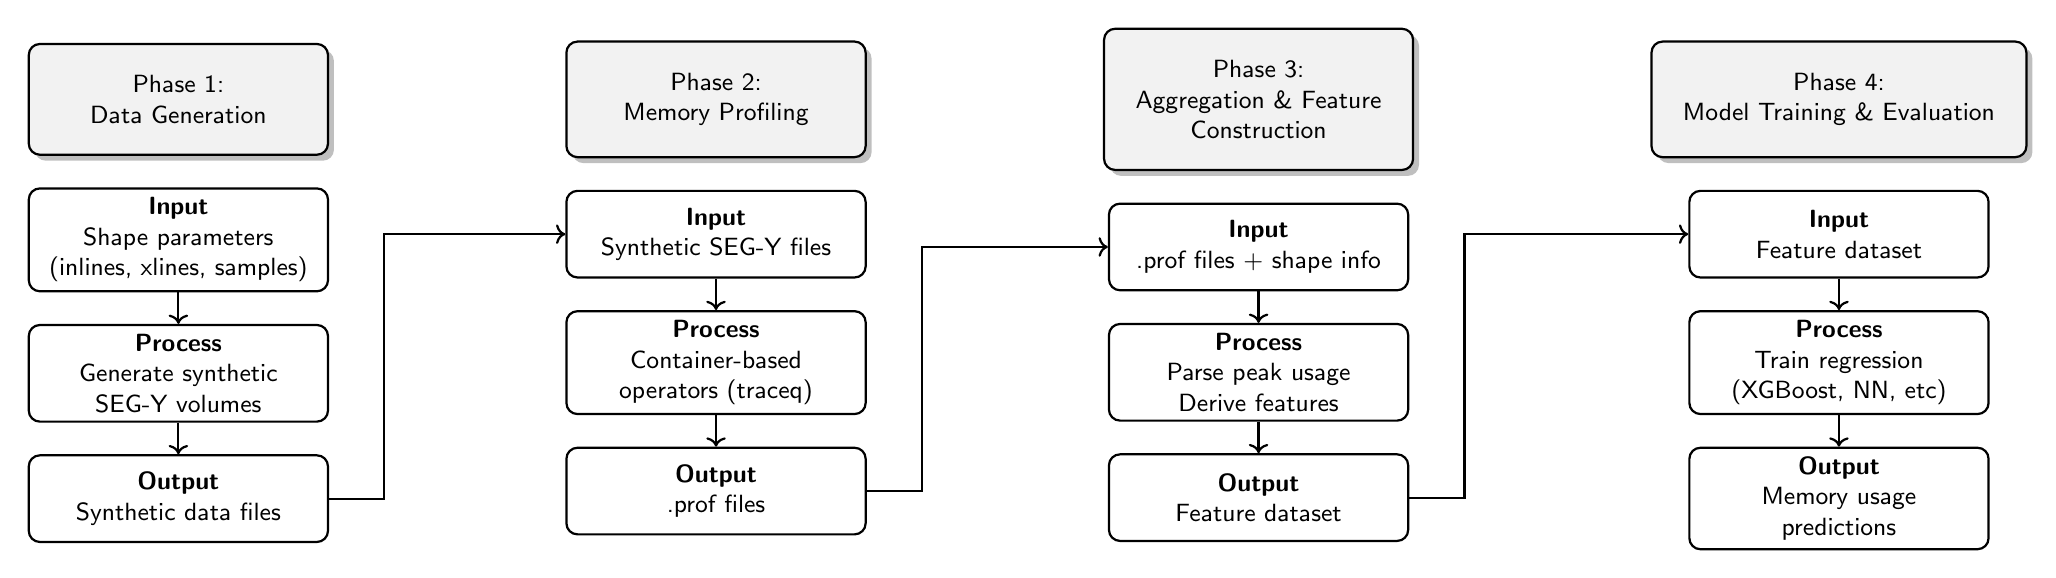
\begin{tikzpicture}[
            font=\sffamily\small,
            phase/.style={
                draw=black,
                thick,
                fill=gray!10,
                rectangle,
                rounded corners,
                drop shadow,
                align=center,
                minimum width=3.8cm,
                inner sep=0.4cm
            },
            box/.style={
                draw=black,
                thick,
                fill=white,
                rectangle,
                rounded corners,
                align=center,
                minimum width=3.8cm,
                minimum height=1.1cm
            },
            arrow/.style={
                ->,
                thick
            },
            node distance=0.4cm and 0.8cm
        ]

            % Phase 1: Data Generation
            \node[phase] (phase1) {Phase 1:\\Data Generation};
            \node[box, below=of phase1] (p1input) {\textbf{Input}\\Shape parameters\\(inlines, xlines, samples)};
            \node[box, below=of p1input] (p1process) {\textbf{Process}\\Generate synthetic\\SEG-Y volumes};
            \node[box, below=of p1process] (p1output) {\textbf{Output}\\Synthetic data files};

            \draw[arrow] (p1input) -- (p1process);
            \draw[arrow] (p1process) -- (p1output);

            % Phase 2: Memory Profiling
            \node[phase, right=3cm of phase1] (phase2) {Phase 2:\\Memory Profiling};
            \node[box, below=of phase2] (p2input) {\textbf{Input}\\Synthetic SEG-Y files};
            \node[box, below=of p2input] (p2process) {\textbf{Process}\\Container-based\\operators (traceq)};
            \node[box, below=of p2process] (p2output) {\textbf{Output}\\.prof files};

            \draw[arrow] (p2input) -- (p2process);
            \draw[arrow] (p2process) -- (p2output);
            \draw[arrow] (p1output.east) -- ++(0.7,0) |- (p2input.west);

            % Phase 3: Feature Aggregation
            \node[phase, right=3cm of phase2] (phase3) {Phase 3:\\Aggregation \& Feature\\Construction};
            \node[box, below=of phase3] (p3input) {\textbf{Input}\\.prof files + shape info};
            \node[box, below=of p3input] (p3process) {\textbf{Process}\\Parse peak usage\\Derive features};
            \node[box, below=of p3process] (p3output) {\textbf{Output}\\Feature dataset};

            \draw[arrow] (p3input) -- (p3process);
            \draw[arrow] (p3process) -- (p3output);
            \draw[arrow] (p2output.east) -- ++(0.7,0) |- (p3input.west);

            % Phase 4: Model Training
            \node[phase, right=3cm of phase3] (phase4) {Phase 4:\\Model Training \& Evaluation};
            \node[box, below=of phase4] (p4input) {\textbf{Input}\\Feature dataset};
            \node[box, below=of p4input] (p4process) {\textbf{Process}\\Train regression\\(XGBoost, NN, etc)};
            \node[box, below=of p4process] (p4output) {\textbf{Output}\\Memory usage\\predictions};

            \draw[arrow] (p4input) -- (p4process);
            \draw[arrow] (p4process) -- (p4output);
            \draw[arrow] (p3output.east) -- ++(0.7,0) |- (p4input.west);

        \end{tikzpicture}
    }
    \caption{Schematic of the memory prediction pipeline. It includes synthetic data generation, containerized profiling, feature extraction, and regression model training.}
    \label{fig:pmc_datapipeline}
\end{figure}
%\section{Experimental Setup}
%\label{sec:pmc-experimental-setup}
%
%Software and Hardware Environment: Experiments were conducted in a Python-based HPC environment.
%The code is executed on [describe hardware – e.g., “a compute node with 256 GB RAM and 2× Intel Xeon CPUs”] or a similar platform, ensuring that even the largest test case can be run without swapping.
%We utilize Python libraries including NumPy for synthetic data generation, and TraceQ (a custom memory profiling tool) to measure memory consumption.
%TraceQ hooks into the process to log memory usage over time; from its output we extract the peak memory usage (maximum resident set size) during each run.
%This peak corresponds to the “Max Memory” metric reported by cluster job monitors (https://hpc.ncsu.edu/Documents/memory.php#:~:text=Max%20Memory%20%3A%20%20,08%20MB), which is the key quantity for resource planning.
%By capturing peak memory, we ensure our predictions aim at the worst-case usage during execution.
%
%Target Algorithm and Implementation: We focus on a representative tensor-based workload from seismic data processing.
%In particular, the code under test could be a function that takes a multi-dimensional seismic array (e.g., a 3D volume) and performs some compute-intensive operation (such as filtering, FFT-based processing, or attribute calculation).
%The specifics of the algorithm (e.g. complexity) are less important than its memory usage behavior.
%We treat it as a fixed “black box” whose memory footprint we want to predict.
%This function is invoked repeatedly with different input array shapes.
%All other factors (code path, data type, etc.) are held constant to isolate the effect of input shape on memory.
%
%Synthetic Dataset Generation: To train our models, we generated a synthetic dataset of input shapes and observed memory usages.
%We varied the input tensor dimensions systematically to cover a broad range of sizes.
%For example, for a 3D workload, we might vary depth, height, and width across realistic ranges (small, medium, large) and sample combinations of these.
%We ensured the synthetic shapes span from very small inputs (to observe baseline memory usage and any fixed overhead) up to near the upper limits of what the hardware could handle (to observe how memory scales at the high end).
%Each unique shape configuration was run through the target algorithm, and TraceQ recorded its peak memory.
%This process yields a labeled dataset: (features = shape metrics, target = memory).
%We repeated each measurement multiple times to verify consistency (minimal run-to-run variance in memory, which we indeed observed, indicating a deterministic memory pattern for given shapes).
%The synthetic approach allows gathering ample data (including extreme cases that might not appear in real datasets) under controlled conditions, which is ideal for training the more data-hungry models like neural nets.
%
%• Real-World Dataset (F3 Seismic) for Validation: In addition to synthetic data, we evaluated our models on a real seismic dataset – the Netherlands F3 block.
%The F3 dataset is a 3D seismic volume of size approximately 255 × 901 × 601 (depth × inline × crossline) (https://www.researchgate.net/figure/The-size-of-Netherlands-F3-dataset-is-255-901-601-depth-crossline-inline_fig3_373406803), totaling on the order of 138 million samples.
%This large volume is representative of high-end workload sizes in our domain.
%We ran the same target algorithm on the F3 data (and subsets or downsampled versions of it, if needed) to gather memory usage in practice.
%The F3 runs serve as an independent test: they allow us to see if models trained on synthetic patterns can generalize to a real-case scenario with a specific shape (and possibly slight differences, like the presence of geologic structures in the data, though that shouldn’t affect memory).
%In our experiments, the F3 full volume and several sub-volumes (for instance, splitting the volume into halves or quarters) were used as test points to evaluate prediction accuracy on real data shapes that were not explicitly in the training set.
%
%Memory Profiling Process: For each experiment (each input shape), we use TraceQ to record memory usage over the runtime of the algorithm.
%We extract the peak memory usage observed.
%This peak is our ground-truth label for the learning models.
%By focusing on peak, we inherently capture the worst-case memory requirement – exactly what needs to be reserved in an HPC job.
%We also note the timing of when the peak occurs (e.g., at a particular stage of the algorithm), though for modeling we only use the peak value.
%The overhead of TraceQ is negligible, and it provides high-resolution memory tracking, which gave us confidence in the accuracy of our measurements (within a few MB). Each shape configuration’s run is isolated (we ensured no other heavy processes on the node, memory was freed between runs, etc.).
%
%Training, Testing, and Validation Strategy: We split our collected data into a training set and a test set.
%The training set (mostly synthetic cases) is used to fit the models.
%We employed k-fold cross-validation on the training set to tune model hyperparameters (for example, to select the polynomial degree or tree depth that yields the best validation score).
%The held-out test set includes some synthetic shapes (to evaluate interpolation performance) and the real F3 cases as separate test points (to evaluate extrapolation or at least interpolation at a larger scale).
%Model performance is quantified using standard regression metrics like Mean Squared Error (MSE) and Coefficient of Determination (R²) on the test set.
%However, given our practical goal, we pay special attention to prediction bias: a model that consistently underestimates memory, even by a small percentage, is considered riskier than one that overestimates by a moderate amount.
%To capture this, we introduced a custom scoring metric that penalizes under-predictions more heavily than over-predictions.
%In practice, this could be a weighted error or a custom loss function where if predicted memory < actual memory, the penalty is amplified.
%We used this score to rank the models for “safety.” The metric reflects the fact that an underestimation could lead to a job crash (which is far worse than overestimation leading to some idle reserved memory) (https://pmc.ncbi.nlm.nih.gov/articles/PMC9906793/#:~:text=While%20these%20resource%20requirements%20are,waiting%20time%20for%20submitted%20jobs).
%Throughout training, we monitored this metric as well, and in model selection, we gave priority to models with little to no underestimation on validation data.
%
%Summary of Experimental Setup: In summary, our experiments involved hundreds of runs of the seismic algorithm with varying input shapes, automated memory tracking, and offline training of various predictive models.
%The combination of synthetic exhaustive sampling and real-case testing provides a robust assessment of whether input shape alone suffices to predict memory.
%Next, we present the results, including visual comparisons of predicted vs. actual memory usage and error analysis for each model type.
%
\section{Experimental Results}
\label{sec:pmc-results}

This chapter presents the results of predicting memory consumption from seismic input shapes.
The results are evaluated into five main categories: (i) memory and execution-time profiling, (ii) model performance overview, (iii) feature selection experiments, (iv) data reduction studies, and (v) cross-operator comparisons.
Each section provides insights into the memory usage patterns of the seismic operators, the performance of regression models, the impact of feature selection, and the robustness of the models under data scarcity.
All analyses and experiment results are located in the \texttt{experiment} directory of the project repository~\cite{delucca2025experiment2results}.

\subsection{Experiment Outputs Overview}
\label{subsec:pmc-results-experiment-outputs-overview}

This section introduces the operators under study, highlights the main experimental goals, and outlines key data artifacts.
The final segments of the pipeline generated five distinct \ac{CSV} files that consolidate memory usage measurements, model evaluations, feature selection outcomes, and data-reduction experiments.
These artifacts form the basis for subsequent analyses in the following sections.

\vspace{1em}
\noindent
\textbf{Operators and Experimental Goals.}
Three operators were evaluated: Envelope, \ac{GST3D}, and the 3D Gaussian Filter.
All three process seismic data volumes and exhibit distinct computational traits.
The primary objective involved modeling their peak \ac{RAM} consumption based on shape parameters (inlines, xlines, and samples), thereby enabling more informed \ac{HPC} resource allocations.

\vspace{1em}
\noindent
\textbf{Data Artifacts.}
The experiment produced five core \ac{CSV} files:
\begin{enumerate}
    \item \emph{profile\_history.csv}:
    Time-series snapshots of \ac{RSS} and corresponding timestamps.
    Each row represents one data capture during an operator’s execution.
    \item \emph{profile\_summary.csv}:
    Aggregated statistics about peak memory usage and execution time per input volume.
    This file stores the mean, standard deviation, minimum, and maximum peak memory usage, along with average runtimes and related descriptors.
    \item \emph{model\_metrics.csv}:
    Performance metrics (\ac{RMSE}, \ac{MAE}, $R^2$, accuracy, and an overall score) for each trained regression model.
    It also includes arrays of residuals, predicted values, and ground truths for deeper error analysis.
    \item \emph{feature\_selection.csv}:
    Results of experiments that use different subsets of features to predict memory usage.
    Each row documents the selected features, model configuration, and associated performance (\ac{RMSE}, \ac{MAE}, $R^2$, accuracy, and score).
    \item \emph{data\_reduction.csv}:
    Outputs from varying the number of training samples.
    The file compares performance metrics across multiple training-set sizes to study model robustness under data scarcity.
\end{enumerate}

\vspace{1em}
\noindent
\textbf{Shape Configurations.}
The synthetic datasets spanned multiple \ac{3D} dimensions.
Volumes ranged from smaller shapes (e.g., $100$ $\times$ $100$ $\times$ $100$) to significantly larger ones close to memory limits of the test system.
Each operator was executed for these volumes to capture comprehensive memory-profiling data.
This systematic approach reveals how memory usage and execution time evolve as the number of traces or samples grows.

\vspace{1em}
\noindent
\textbf{Chapter Roadmap.}
Section~\ref{sec:pmc-results-memory-and-execution-time-profiling} first presents how memory usage behaved during operator runs and highlights the aggregated profiling statistics.
Subsequent sections detail model performance across regression approaches, emphasizing how different features and training subsets affect accuracy.
The final portion compares Envelope, \ac{GST3D}, and Gaussian Filter side by side to underscore differences and provide practical insights for \ac{HPC} scheduling.


\section{Memory and Execution-Time Profiling}
\label{sec:pmc-results-memory-and-execution-time-profiling}

This section examines how memory usage and execution time scale with input volume and seismic dimension sizes for Envelope, \ac{GST3D}, and the Gaussian Filter.

\subsection{Linear Trends and Variability}
\label{subsec:linear-trends-and-variability}

Figure~\ref{fig:peak_memory_facet} show that average peak memory usage grows linearly with increasing volume for Envelope, \ac{GST3D}, and Gaussian Filter.
A higher \ac{CV} is observed for smaller volumes, whereas larger volumes yield more stable, yet higher, memory consumption.

\begin{figure*}[htbp]
    \centering
    \begin{subfigure}[t]{0.49\textwidth}
        \centering
        \includegraphics[width=\textwidth]{assets/images/05/peak_memory_by_volume_envelope}
        \caption{Envelope: Smaller volumes exhibit higher variability,
            while larger volumes show a consistent linear growth.}
    \end{subfigure}
    \hfill
    \begin{subfigure}[t]{0.49\textwidth}
        \centering
        \includegraphics[width=\textwidth]{assets/images/05/peak_memory_by_volume_gst3d}
        \caption{\ac{GST3D}: Exhibits a steeper slope relative to Envelope.}
    \end{subfigure}
    \hfill
    \begin{subfigure}[t]{0.49\textwidth}
        \centering
        \includegraphics[width=\textwidth]{assets/images/05/peak_memory_by_volume_gaussian-filter}
        \caption{Gaussian Filter: Memory consumption scales linearly,
            though less steeply than \ac{GST3D}.}
    \end{subfigure}
    \caption{Peak memory usage by volume for three operators: Envelope, \ac{GST3D}, and the Gaussian Filter.
    Memory usage grows linearly with volume, with larger volumes requiring more resources.}
    \label{fig:peak_memory_facet}
\end{figure*}

Figure~\ref{fig:ex_peak_mu_facet} indicate that execution time and memory usage both rise in near-linear fashion across all operators.
Similarly, figure~\ref{fig:execution_time_by_volume_facet} confirm that execution time correlates strongly with volume for each seismic algorithm evaluated.

\begin{figure*}[htbp]
    \centering
    \begin{subfigure}[t]{0.49\textwidth}
        \centering
        \includegraphics[width=\textwidth]{assets/images/05/cross_execution_time_by_volume}
        \caption{Execution time by volume for Envelope, \ac{GST3D}, and the Gaussian Filter.}
    \end{subfigure}
    \hfill
    \begin{subfigure}[t]{0.49\textwidth}
        \centering
        \includegraphics[width=\textwidth]{assets/images/05/cross_peak_memory_by_volume}
        \caption{Peak memory usage by volume for Envelope, \ac{GST3D}, and the Gaussian Filter.}
    \end{subfigure}
    \hfill
    \begin{subfigure}[t]{0.49\textwidth}
        \centering
        \includegraphics[width=\textwidth]{assets/images/05/cross_operator_memory_scaling_factor}
        \caption{Linear-fit slope of memory usage vs volume by operator.
        Higher values imply more rapid growth with increasing volume.}
    \end{subfigure}
    \caption{Peak memory usage and execution time by volume for Envelope, \ac{GST3D}, and the Gaussian Filter.
    Both metrics exhibit a clear linear trend, with larger volumes requiring more resources.}
    \label{fig:ex_peak_mu_facet}
\end{figure*}

\begin{figure*}[htbp]
    \centering
    \begin{subfigure}[t]{0.49\textwidth}
        \includegraphics[width=\textwidth]{assets/images/05/execution_time_by_volume_envelope}
    \end{subfigure}
    \hfill
    \begin{subfigure}[t]{0.49\textwidth}
        \centering
        \includegraphics[width=\textwidth]{assets/images/05/execution_time_by_volume_gst3d}
    \end{subfigure}
    \hfill
    \begin{subfigure}[t]{0.49\textwidth}
        \centering
        \includegraphics[width=\textwidth]{assets/images/05/execution_time_by_volume_gaussian-filter}
    \end{subfigure}
    \caption{Execution time by volume for Envelope, \ac{GST3D}, and the Gaussian Filter.
    The chart shows a clear linear trend, with larger volumes requiring more time to process.}
    \label{fig:execution_time_by_volume_facet}
\end{figure*}

\subsection{Execution Time Distributions and Scaling Factor}
\label{subsec:execution-time-distributions-and-scaling}

Figure~\ref{fig:execution_time_distribution_facet} depict right-skewed distributions of run durations, indicative of gamma- or lognormal-like behavior.
Most runs complete quickly, but outliers at the high end extend the tail.

\begin{figure*}[htbp]
    \centering
    \begin{subfigure}[t]{0.49\textwidth}
        \centering
        \includegraphics[width=\textwidth]{assets/images/05/execution_time_distribution_envelope}
    \end{subfigure}
    \hfill
    \begin{subfigure}[t]{0.49\textwidth}
        \centering
        \includegraphics[width=\textwidth]{assets/images/05/execution_time_distribution_gst3d}
    \end{subfigure}
    \hfill
    \begin{subfigure}[t]{0.49\textwidth}
        \centering
        \includegraphics[width=\textwidth]{assets/images/05/execution_time_distribution_gaussian-filter}
    \end{subfigure}
    \caption{Execution time distributions for Envelope, \ac{GST3D}, and the Gaussian Filter.
    The distribution shows a clear left skew, with most runs completing quickly.}
    \label{fig:execution_time_distribution_facet}
\end{figure*}

Figure~\ref{fig:ex_peak_mu_facet} shows a bar chart of the linear-fit coefficients (slopes) for each operator’s average peak \ac{RAM} usage vs volume.
\ac{GST3D} exhibits the largest slope, reflecting more elaborate data structures and intermediate buffers for discontinuity detection.
Envelope has a moderate slope, whereas Gaussian Filter is the least steep, indicating more incremental memory use.

\subsection{Dimension-Specific and Time-Progression Analysis}
\label{subsec:dimension-specific-and-time-progression-analysis}

Figure~\ref{fig:memory_usage_by_configuration_envelope} show dimension-specific breakdowns (inlines, xlines, samples) for the Envelope operator, confirming that each dimension contributes similarly to overall memory usage.
Also, figure~\ref{fig:memory_usage_by_configuration_envelope} illustrate that higher memory consumption correlates with longer run durations for the Envelope operator.

\begin{figure*}[htbp]
    \centering
    \begin{subfigure}[t]{0.49\textwidth}
        \centering
        \includegraphics[width=\textwidth]{assets/images/05/memory_usage_by_configuration_envelope}
        \caption{Memory usage by inlines, xlines, and samples for Envelope.
        All dimensions contribute equally to memory consumption.}
    \end{subfigure}
    \hfill
    \begin{subfigure}[t]{0.49\textwidth}
        \centering
        \includegraphics[width=\textwidth]{assets/images/05/execution_time_vs_memory_envelope}
        \caption{Execution time vs memory usage for Envelope.}
    \end{subfigure}
    \hfill
    \begin{subfigure}[t]{0.49\textwidth}
        \centering
        \includegraphics[width=\textwidth]{assets/images/05/memory_usage_inlines_xlines_samples_heatmap_envelope}
        \caption{Memory usage heatmap by inlines, xlines, and samples for Envelope.}
    \end{subfigure}
    \caption{Memory usage and execution time analysis for the Envelope operator.}
    \label{fig:memory_usage_by_configuration_envelope}
\end{figure*}

Violin charts in Figure~\ref{fig:memory_usage_distribution} illustrate memory usage fluctuations over time for each operator.
Envelope shows wider distributions, indicating more gradual ramps and fluctuations.
Gaussian Filter and \ac{GST3D} reach stable peak memory usage more rapidly, resulting in thinner violins.

\begin{figure*}[htbp]
    \centering
    \begin{subfigure}[t]{0.49\textwidth}
        \centering
        \includegraphics[width=\textwidth]{assets/images/05/memory_usage_distribution_envelope}
    \end{subfigure}
    \hfill
    \begin{subfigure}[t]{0.49\textwidth}
        \centering
        \includegraphics[width=\textwidth]{assets/images/05/memory_usage_distribution_gst3d}
    \end{subfigure}
    \hfill
    \begin{subfigure}[t]{0.49\textwidth}
        \centering
        \includegraphics[width=\textwidth]{assets/images/05/memory_usage_distribution_gaussian-filter}
    \end{subfigure}
    \caption{Violin charts of memory usage over time for Envelope, \ac{GST3D}, and the Gaussian Filter.
    Envelope exhibits wider distributions, while \ac{GST3D} and the Gaussian Filter show more stable memory usage.}
    \label{fig:memory_usage_distribution}
\end{figure*}

Figure~\ref{fig:memory_usage_by_configuration_envelope} shows a heatmap indicating that memory usage rises uniformly across the three dimensions.
Figure~\ref{fig:inline_xline_memory_usage_progression_envelope} confirm that Envelope ramps more uniformly in time.

\begin{figure}[htbp]
    \centering
    \includegraphics[width=\textwidth]{assets/images/05/inline_xline_memory_usage_progression_envelope}
    \caption{Memory usage progression by inlines and xlines for Envelope.}
    \label{fig:inline_xline_memory_usage_progression_envelope}
\end{figure}

\subsection{Memory Safety Margins}
\label{subsec:memory-safety-margins}

Figure~\ref{fig:memory_safety_margins} highlight the difference between average and 95th-percentile memory usage across tested volumes.
Envelope and \ac{GST3D} can exhibit large gaps in memory usage, which indicates that some runs exceed the typical allocation by a significant margin.
Isolating experiments via containerization did not fully eliminate kernel-level optimizations or other system effects that cause these outliers.

\begin{figure*}[htbp]
    \centering
    \begin{subfigure}[t]{0.49\textwidth}
        \centering
        \includegraphics[width=\textwidth]{assets/images/05/memory_safety_margin_envelope}
    \end{subfigure}
    \hfill
    \begin{subfigure}[t]{0.49\textwidth}
        \centering
        \includegraphics[width=\textwidth]{assets/images/05/memory_safety_margin_gst3d}
    \end{subfigure}
    \hfill
    \begin{subfigure}[t]{0.49\textwidth}
        \centering
        \includegraphics[width=\textwidth]{assets/images/05/memory_safety_margin_gaussian-filter}
    \end{subfigure}
    \caption{Memory safety margins for Envelope, \ac{GST3D}, and the Gaussian Filter.
    The 95th percentile often surpasses the average, suggesting occasional high-memory runs.}
    \label{fig:memory_safety_margin}
\end{figure*}

\subsection{Dimension Correlations}
\label{subsec:dimension-correlations}

Figure~\ref{fig:memory_vs_dimensions_pairplot_gst3d} presents a pairplot examining \ac{GST3D} memory usage alongside inlines, xlines, and samples.
Positive slopes confirm that higher dimensions correlate with increased memory.
Negative slopes among dimension--dimension cells primarily reflect the experimental test grid, where large values in one dimension often paired with smaller values in another.
Despite these trade-offs, the net memory footprint rose whenever any dimension increased significantly.

\begin{figure}[htbp]
    \centering
    \includegraphics[width=0.9\textwidth]{assets/images/05/memory_vs_dimensions_pairplot_gst3d}
    \caption{Pairplot of memory usage vs inlines, xlines, and samples for \ac{GST3D}.
    Larger shapes yield higher \ac{RAM} usage.}
    \label{fig:memory_vs_dimensions_pairplot_gst3d}
\end{figure}

\subsection{Summary of Observed Resource Usage}
\label{subsec:resource-usage-summary}

Table~\ref{tab:operator_summary_aggregates} summarizes key metrics for each operator, including tested volume ranges, peak memory usage ranges, and execution time ranges.
It combines the raw data into concise statistics that highlight how quickly memory usage and runtime escalate with increasing volume.

\begin{table}[htbp]
    \centering
    \begin{tabular}{lcccc}
        \hline
        \textbf{Operator} & \textbf{Volume Range} & \textbf{Peak Mem. Usage (GB)} & \textbf{Exec. Time (s)} \\ \hline
        Envelope &
        $10^6 \!\to\! 6.4\times10^7$ &
        0.10 -- 1.76 &
        0.0106 -- 0.5025 \\
        \ac{GST3D} &
        $10^6 \!\to\! 2.7\times10^7$ &
        0.31 -- 6.12 &
        0.2475 -- 7.75 \\
        Gaussian Filter &
        $10^6 \!\to\! 6.4\times10^7$ &
        0.10 -- 0.57 &
        0.0232 -- 1.22 \\
        \hline
    \end{tabular}
    \caption{Resource usage summary for Envelope, \ac{GST3D}, and Gaussian Filter.
    Volumes are specified in number of samples (e.g., $1000000$ = $10^6$).
    Memory usage values appear in GB, and times appear in seconds.
    Each range denotes the minimum and maximum observed across tested volumes.}
    \label{tab:operator_summary_aggregates}
\end{table}

Table~\ref{tab:operator_summary_aggregates} confirms that \ac{GST3D} consistently displays the highest memory usage for similarly sized volumes, with Envelope at an intermediate level, and the Gaussian Filter at a lower bound, though it still scales markedly with volume.
Overall, both memory and execution time exhibit near-linear growth, reinforcing the importance of volume-driven resource estimation.
These findings guide \ac{HPC} users to anticipate how large seismic datasets will stress system \ac{RAM} and runtime allocations, especially in scenarios with competing workloads.


\section{Model Performance Overview}
\label{sec:pmc-results-model-performance-overview}

%- chart assets/images/05/actual_vs_predicted_by_model.pdf shows the results per model and operator. It compares the actual and predicted values. It is clear that most of the models got a pretty good result, but a few of those we can highlight. Namely linear regression,xgboost,and elastic net went pretty well for all models
%- chart assets/images/05/residual_vs_predicted.pdf shows clearly that most models got pretty low residuals. Really close to 0. A few models for a few operators went pretty bad, specially for the gst3d operator
%- chart assets/images/05/cross_model_r2_bar.pdf shows all models r2 scores per operator. We can see that the neural network was the only that perform poorly on gst3d, and we can corroborate the results from the previous chart, that the linear regression, xgboost, and elastic net were the best models
%- charts assets/images/05/score_by_model_envelope.pdf, assets/images/05/score_by_model_gst3d.pdf, assets/images/05/score_by_model_gaussian_filter.pdf show the score for each model per operator. We can see that the best model varies depending on the operator, but we have many models that are really close. For envelope the best model was gradient boost, with a score of 2,579 while for gaussian filter many models performed well, being linear regression the best with a score of 2,904. For gst3d the top score was 2,970 for the decision tree model
%- chart assets/images/05/best_model_per_operator.pdf shows that in a single chart (what was mentioned above)


\section{Feature Selection Experiments}
\label{sec:pmc-results-feature-selection-experiments}


\section{Data Reduction Studies}
\label{sec:pmc-results-data-reduction-studies}


\section{Summary of Findings}
\label{sec:pmc-results-summary-of-findings}
\section{Conclusion}
\label{sec:pmc-conclusion}

This chapter explored the relationship between seismic input shapes and operator-specific memory consumption, focusing on three major processing routines—Envelope, \ac{GST3D}, and Gaussian Filter—and detailed how varying sample sizes, selected features, and modeling pipelines affect predictive accuracy.
Several salient findings emerged:

\begin{itemize}
    \item \textbf{Linear Volume Dependence and Operator Sensitivity.}
    All operators demonstrated a near-linear escalation in peak \ac{RAM} usage with respect to total input volume (\( \text{inlines} \times \text{xlines} \times \text{samples} \)).
    \ac{GST3D} remained the most sensitive, displaying a steeper volume-based slope compared to Envelope and Gaussian Filter.
    Envelope and Gaussian Filter, by contrast, showed comparatively gentler linear relationships, suggesting that their computational kernels rely less on large intermediate buffers.

    \item \textbf{Feature Selection and the Predominance of Volume.}
    Systematic removal of shape-derived features (e.g., diagonal length, surface area, ratio transformations) underscored that \emph{volume} alone captures most of the variance in peak memory usage.
    Even advanced transformations (logarithmic or polynomial terms) contributed only marginal improvements once volume was included.
    \ac{GST3D} occasionally benefited from additional parameters (e.g., diagonal length), but not enough to outweigh the straightforward predictive power of volume.

    \item \textbf{Model Performance and Robustness.}
    Across nine regression approaches, simpler or regularized methods—like \ac{Linear Regression}, Elastic Net, and decision-tree ensembles—performed well, achieving \(R^2 \approx 0.99\) or higher in many configurations.
    Specifically:
    \begin{itemize}
        \item \textbf{Envelope}: Gradient Boosting offered top-level accuracy, though multiple models clustered in the same performance range.
        \item \textbf{\ac{GST3D}}: Decision Trees (and some ensemble variants) captured memory usage reliably but exhibited greater sensitivity to missing data in the mid-volume range.
        \item \textbf{Gaussian Filter}: \ac{Linear Regression} proved sufficient, reinforcing that this operator’s memory footprint aligns closely with volume.
    \end{itemize}
    All methods exhibited mild to moderate right-skew in their residual distributions, yet \ac{RMSE} and \ac{MAE} remained low once mid- and upper-bound volumes were adequately represented.

    \item \textbf{Subsampling and Data Requirements.}
    Pruning the dataset to 30–40 shape configurations preserved high $R^2$ values, indicating that modest sampling—particularly anchored at small and large volumes—enables accurate modeling.
    \ac{GST3D} showed slightly larger degradation at smaller sample counts, reflecting its more complex intermediate data allocations.
    By contrast, Envelope and Gaussian Filter sustained robust predictions with moderate data reduction.
\end{itemize}

Overall, Chapter~\ref{sec:pmc-results} establishes that:
\begin{enumerate}
    \item \emph{Volume is the primary explanatory feature} for predicting peak memory usage, with additional variables offering only minor gains.
    \item Simple or linear-in-spirit regressors often suffice to model Envelope and Gaussian Filter, while \ac{GST3D} can benefit from tree-based methods if data coverage in the mid-volume range is adequate.
    \item A sample size of approximately 30–40 shape configurations provides a practical lower bound for stable memory prediction, making data collection efforts more tractable for real-world \ac{HPC} scenarios.
\end{enumerate}

With these findings, we have a clearer framework for implementing memory-aware chunking strategies: one can rely on volume-based models (potentially augmented by minimal shape features) and still maintain accurate peak \ac{RAM} estimates, even with relatively small training sets.
The subsequent chapter applies these insights to optimize data-parallel chunking and scheduling decisions for large-scale seismic workloads.
    \chapter{Improving Data Parallelism using Memory-Aware Chunking}
\label{ch:improving-data-parallelism-using-memory-aware-chunking}


\section{Introduction}
\label{sec:mac-introduction}

\DFTODO{Explicar sobre o uso do paralelismo de dados}
\DFTODO{Explicar sobre a importância de se ter um bom balanceamento de carga e como isso pode ser feito.}
\DFTODO{Explicar sobre o uso de chunking para o balanceamento de carga}
\DFTODO{Conectar a seção anterior, falando que é feito tentativa e erro pra definir o tamanho do chunk}
\DFTODO{Explicar sobre a natureza de algoritmos tensoriais e linkar com a sessão anterior que é possível prever o consumo de memória}


\section{Dask Auto-Chunking}
\label{sec:mac-dask-auto-chunking}

\DFTODO{Explicar como o auto-chunking do dask funciona e suas limitações}


\section{Memory-Aware Chunking}
\label{sec:mac-memory-aware-chunking}

\DFTODO{Explicar sobre a proposta de chunking baseado no consumo de memória}


\section{Materials and Methods}
\label{sec:mac-materials-methods}

\DFTODO{Explicar sobre o setup do experimento de um ponto de vista de hardware}
\DFTODO{Explicar sobre o setup do experimento de um ponto de vista de software}
\DFTODO{Descrever o fluxo de execução do experimento}
\DFTODO{Explicar como foi feita a configuração do cluster Dask}
\DFTODO{Descrever os experimentos com chunks diferentes para demonstrar as limitações do Dask auto-chunking}
\DFTODO{Descrever a geração de dados, linkando com a sessão anterior}
\DFTODO{Descrever os algoritmos, linkando com a sessão anterior}
\DFTODO{Descrever as métricas coletadas: tempo de execução, uso máximo de memória, overhead de escalonamento, número de chunks, relação chunk-to-worker, temanho relativo do chunk}
\DFTODO{Descrever as técnicas utilizadas para analisar os dados}
\DFTODO{Linkar com o código fonte}


\section{Experimental Results}
\label{sec:mac-experimental-results}

\DFTODO{Descrever como diferentes formatos de chunk afetam o desempenho}
\DFTODO{Demonstrar e comparar o Memory-Aware Chunking com o Auto-Chunking do Dask}
\DFTODO{Demonstrar e descrever o previsor de melhor tamanho de chunk que foi desenvolvido com base nos resultados}


\section{Conclusion}
\label{sec:mac-conclusion}

\DFTODO{Concluir sobre a importância de se ter um bom balanceamento de carga}
\DFTODO{Explicar e concluir sobre a possibilidade de encontrar o melhor tamanho de chunk baseado no consnumo estimado de memória}
\DFTODO{Discutir as complexidades e próximos passos para integrar facilmente com o Dask}


    \chapter{Conclusion}
\label{ch:conclusion}

\DFTODO{Organizar e escrever a conclusão}

    \bibliographystyle{plain}
    \bibliography{bibliography}

% \appendix
% \chapter{Anexo 1}
% \chapter{Anexo 2}

\end{document}